\documentclass[sigconf]{acmart}

\usepackage{booktabs} % For formal tables

\usepackage[latin1]{inputenc}
\usepackage[T1]{fontenc}
\usepackage{libertine}
\usepackage{graphicx,color,url}
\usepackage[dvips]{epsfig}
\usepackage{verbatim}
\usepackage{tikz}
\usetikzlibrary{shapes,arrows}
\usetikzlibrary{calc,patterns,snakes,decorations.pathmorphing,decorations.markings}
\usetikzlibrary{positioning}
\usepackage{amsmath}
\usepackage{tabularx} % better tables
\usepackage{float}
\setlength{\extrarowheight}{3pt} % increase table row height
\newcommand{\tableheadline}[1]{\multicolumn{1}{c}{\spacedlowsmallcaps{#1}}}
\newcommand{\myfloatalign}{\centering} % to be used with each float for 
%alignment
\usepackage{caption}
\captionsetup{font=small} % format=hang,
\usepackage{subfig}
\usepackage[ruled]{algorithm2e}
%\providecommand{\tabularnewline}{\\}
\usepackage{listings}
\usepackage{color}
\usepackage{graphicx}

%\newcommand{\keywords}[1]{\par\addvspace\baselineskip
%	\noindent\keywordname\enspace\ignorespaces#1}

\definecolor{dkgreen}{rgb}{0,0.6,0}
\definecolor{gray}{rgb}{0.5,0.5,0.5}
\definecolor{mauve}{rgb}{0.58,0,0.82}
\definecolor{gray}{rgb}{0.4,0.4,0.4}
\definecolor{darkblue}{rgb}{0.0,0.0,0.6}
\definecolor{lightblue}{rgb}{0.0,0.0,0.9}
\definecolor{cyan}{rgb}{0.0,0.6,0.6}
\definecolor{darkred}{rgb}{0.6,0.0,0.0}

\lstset{
	basicstyle=\ttfamily\footnotesize,
	columns=fullflexible,
	showstringspaces=false,
	numbers=left,                   % where to put the line-numbers
	numberstyle=\tiny\color{gray},  % the style that is used for the 
	%line-numbers
	stepnumber=1,
	numbersep=5pt,                  % how far the line-numbers are from the code
	backgroundcolor=\color{white},      % choose the background color. You must 
	%add \usepackage{color}
	showspaces=false,               % show spaces adding particular underscores
	showstringspaces=false,         % underline spaces within strings
	showtabs=false,                 % show tabs within strings adding 
	%particular underscores
	frame=none,                   % adds a frame around the code
	rulecolor=\color{black},        % if not set, the frame-color may be 
	%changed on line-breaks within not-black text (e.g. commens (green here))
	tabsize=2,                      % sets default tabsize to 2 spaces
	captionpos=b,                   % sets the caption-position to bottom
	breaklines=true,                % sets automatic line breaking
	breakatwhitespace=false,        % sets if automatic breaks should only 
	%happen at whitespace
	title=\lstname,                   % show the filename of files included 
	%with \lstinputlisting;
	% also try caption instead of title  
	commentstyle=\color{gray}\upshape
}


\lstdefinelanguage{XML}
{
	morestring=[s][\color{mauve}]{"}{"},
	morestring=[s][\color{black}]{>}{<},
	morecomment=[s]{<?}{?>},
	morecomment=[s][\color{dkgreen}]{<!--}{-->},
	stringstyle=\color{black},
	identifierstyle=\color{lightblue},
	keywordstyle=\color{red},
	morekeywords={material, minWidth, maxWidth, width, rotation, type, id, x, 
	y, source, target, version}% list your attributes here
}



% Copyright
%\setcopyright{none}
%\setcopyright{acmcopyright}
%\setcopyright{acmlicensed}
\setcopyright{rightsretained}
%\setcopyright{usgov}
%\setcopyright{usgovmixed}
%\setcopyright{cagov}
%\setcopyright{cagovmixed}


% DOI
\acmDOI{10.1145/nnnnnnn.nnnnnnn}

% ISBN
\acmISBN{978-x-xxxx-xxxx-x/YY/MM}

% Conference
\acmConference[GECCO '19]{the Genetic and Evolutionary Computation Conference 
2019}{July 13--17, 2019}{Prague, Czech Republic}
\acmYear{2019}
\copyrightyear{2019}

%\acmArticle{4}
\acmPrice{15.00}

% These commands are optional
%\acmBooktitle{Transactions of the ACM Woodstock conference}
%\editor{Jennifer B. Sartor}
%\editor{Theo D'Hondt}
%\editor{Wolfgang De Meuter}


\begin{document}
\title{Improved Free Form Evolution for Angry Birds Structures}

  
  \author{Laura Calle}
  \affiliation{%
    \institution{Universidad de Granada}
  }
  \email{laucalle09@gmail.com}

  \author{Juan-Juli\'an Merelo-Guerv\'os, Antonio Mora-Garc�a}
%  \orcid{1234-5678-9012}
  \affiliation{%
    \institution{Universidad de Granada/CITIC}
    \city{Granada,Spain}
    \postcode{18071}
  }
  \email{(jmerelo|amorag)@ugr.es}

  \author{Mario Garc\'ia Valdez}
  \affiliation{%
    \institution{Tecnol\'ogico Nacional de M\'exico}
    \city{Tijuana}
    \state{M\'exico}
    \postcode{22414}
  }
  \email{mario@tectijuana.edu.mx}

\renewcommand{\shortauthors}{Calle et al.}


\begin{abstract}
This paper presents an original approach based on evolutionary
algorithms for building structures that are stable under gravity for
the physics-based puzzle game Angry Birds, with the ultimate objective
of creating Angry Birds levels with the minimum number of constraints.
We have created a custom open source evolutionary computation library
that implement an evolutionary algorithm whose main challenges have
been to design a fitness function that, first, avoids when possible
the time-consuming actual execution of the game, and, then, takes into
account the different ways in which a structure is not sound and
eliminates them.  In order to test the method six experiments have
been carried out, obtaining a variety of stable structures, which is
the first path for the generation of levels that are aesthetically
pleasing as well as playable.
\end{abstract}


 \begin{CCSXML}
% Antonio - I have generated this CSS
<ccs2012>
<concept>
<concept_id>10010147.10010178</concept_id>
<concept_desc>Computing methodologies~Artificial intelligence</concept_desc>
<concept_significance>500</concept_significance>
</concept>
<concept>
<concept_id>10010147.10010178.10010205</concept_id>
<concept_desc>Computing methodologies~Search methodologies</concept_desc>
<concept_significance>300</concept_significance>
</concept>
<concept>
<concept_id>10010147.10010178.10010205.10010206</concept_id>
<concept_desc>Computing methodologies~Heuristic function 
construction</concept_desc>
<concept_significance>500</concept_significance>
</concept>
</ccs2012>
\end{CCSXML}

\ccsdesc[500]{Computing methodologies~Artificial intelligence}
\ccsdesc[300]{Computing methodologies~Search methodologies}
\ccsdesc[500]{Computing methodologies~Heuristic function construction}

\keywords{Search-Based Procedural Content Generator, Evolutionary algorithm, 
Game development, Angry Birds, Level generation}


\maketitle

%
%%%%%%%%%%%%%%%%%%%%%%%%%%%%%%%   INTRODUCTION   %%%%%%%%%%%%%%%%%%%%%%%%%%%%%%%
%
\section{Introduction and problem description}
\label{sec:intro}

\textit{Angry Birds} is a mobile game created by Rovio Entertainment
Corporation. In the game, there is a variety of defensive structures
made out of blocks which protect {\em pigs} from the birds fired by
the player. 
There is an ongoing competition on the generation of this
kind of structures, which is a challenge from several points of view;
most authors \cite{stephenson2016procedural} evolve fixed-form
structures known to be stable.
Simulators are used to test procedurally generated game
content; ours was forked from Science Birds \cite{ferreira2014search}
to produce usable output for an evolutionary algorithm \cite{sciencebirds-adapt}.
In this paper we focus in
the generation of free-form structures in an attempt to enhance
replayability of the game.  Since we are interested in structural
integrity of the generated structures, neither actual gameplay nor
players are taken into account;  we will use a {\em direct
fitness function}, which takes measures directly on the generated
content, a time-consuming procedure since it actually involves
entering the simulator and running it, so we will apply heuristics to
the evolved structures to compute a fitness even before simulation.


The main feature of a stable level is that it is not in motion, so we
will evaluate its steadiness as opposed to its speed as a baseline
$$fitness_{ind} = \frac{1}{|V|}\sum_{i=0}^{b}{V_i} + P_{broken}\cdot(b-|V|)$$
The modified simulator provides the average magnitude of velocity for
each block, a set noted as $V$.  The number of blocks in an individual
is $b$, used to calculate .  the number of broken blocks and apply a
penalization to invalid levels ($P_{broken} = 100$).  Since in-game
simulation is a time consuming process, we will skip some levels based
on indicators such as its distance to the ground, the number of
overlapping blocks and the number of blocks broken during the
simulation. In later experiments height is also taken into account
\cite{DBLP:conf/evoW/CalleGGV19}.

For representation, we aim at flexible and simple structures to allow
a less directed search.  Individuals are composed by an unordered,
variable length list of blocks defined by their type (shape and size),
position and rotation. This new representation needed a new, open
source, evolutionary computation framework \cite{ab-level}.


%************************************************
\section{Experimentation and Results}\label{ch:res}

After the initial exploration of free form evolution in
\cite{DBLP:conf/evoW/CalleGGV19}, there were two main problems: first,
the time it took to enter the simulator and obtain the speed of the
blocks; this is an implementation-level issue, but it had influence on
the number of generations we could actually employ. Thus, in this new
experiment, which we called E5, we will use Box2D
\cite{catto2011box2d}, the physics engine used in the original game, adjusted
the parameters so this simulation and the game behave in the same
way. Execution time drastically dropped from 5 hours to less than 20 minutes on average, even running
more generations in the process.
Lower execution time allowed us to perform more operations like penalizing
not only the distance to the ground but also the \textit{gaps} in the
Y-axis, which will make objects drop and maybe break.
This will encourage individuals to grow vertically and not only horizontally
like in previous experiments.
This changes the fitness function, so we
will have to compare by the actual obtained structure. %, one of which is
%shown in Figure \ref{f:e5}.

 \begin{figure}
 	\centering
 	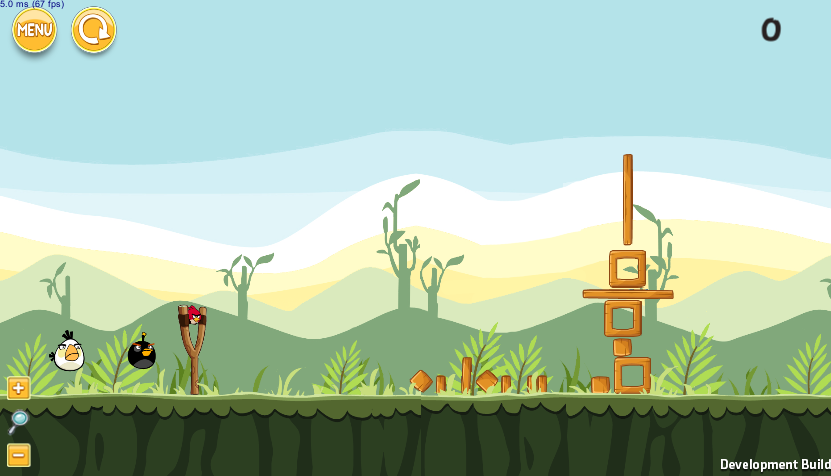
\includegraphics[scale=0.3]{E5.png}
 	\caption{One of the solutions from Experiment 5}\label{f:e5}
      \end{figure}

In general, this penalization of gaps creates a faster path to higher stable
structures.
Still, it led to mostly flat structures with 
some higher block in unstable positions, which
are structurally solid, but not interesting.
One of the stable results is shown in Figure \ref{f:e5}.
% Something more should have to be commented on these results - JJ
% Like this part down here? - Laura

Observing results from the previous experiment we realized that what
evolution found was that laying many blocks on the ground was enough
to get a high fitness: the average speed was decreased and it will
place unstable blocks to cover gaps in Y-axis. Even if those blocks just
free-fall and break, a high amount of static block will compensate.
In order to correct this behaviour we changed the 
fitness function to take into account the fastest moving object.
That way, other blocks will not mask the fact that there are unstable elements
being placed in the level. 
Additionally, we initialized levels including one of a list of pre configured
blocks (disposed as in \cite{ferreira2014search}) in addition to the random initialization used until now.
$$fitness_{indV2} = \max{(V)}$$

%This makes the fitness value depends on just one gene, although it can be a
%different one each time. The improvement of solutions to find acceptable ones
%slowed down % This would have to be proved by a chart
Again, with a different fitness function we cannot compare the fitness
value with the rest of the experiments. One of the results shown in 
Figure \ref{f:e6}. The results were in general more stable and complex than
the ones obtained with the previous fitness function.
 \begin{figure}
 	\centering
 	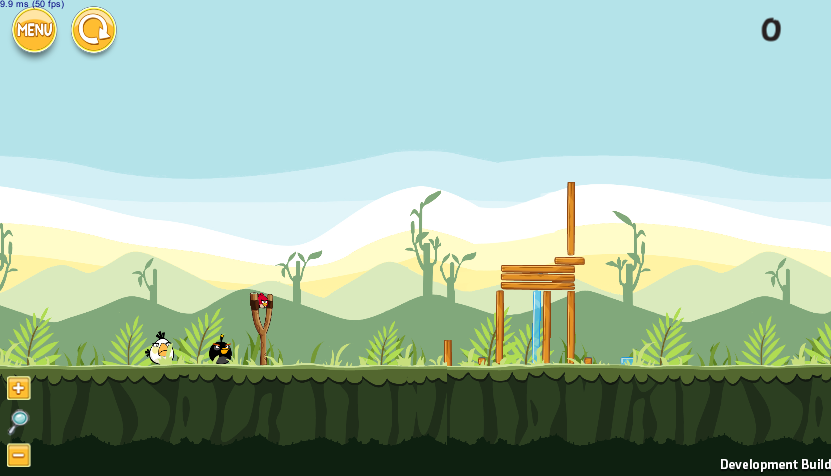
\includegraphics[scale=0.3]{E6.png}
 	\caption{One of the solutions from Experiment 6}\label{f:e6}
 \end{figure}


 %Again, you can't simply show a single figure as a result. Maybe show
 %average height, or several best solutions. And always reference the
 %figure - JJ
 % Problem here is that most of the structures actually fall - Laura
%************************************************



%%%%%%%%%%%%%%%%%%%%%%%%%%%%%  CONCLUSIONS  %%%%%%%%%%%%%%%%%%%%%%%%%%%%
%
\section{Conclusions and Future Work} 
\label{sec:conclusions}

This paper was developed with
objective of exploring the expressiveness and variability of 
SBPCG with evolutionary techniques
and producing stable structures under gravity.

For this aim we have implemented an Evolutionary Algorithm able to optimize 
level structures to meet this criteria. 
The method studied was
sufficiently general and flexible to draw some conclusions about the
topic. SBPCG methods are a potential good solution to offline content
generation but it requires a great amount of problem-specific
knowledge. 
The more rules the author adds, results tend to be 
variations of the same idea. However,
a lack of knowledge
will lead to unexpected outcomes.
In our case, the fitness function used the 
stability of the structure and only considered other features 
to ensure the levels would be valid.

The main issue is how we define levels and how the definition %of level 
plays with the paths of evolution.
Producing stable structures under gravity was effectively
achieved, but the consequence of evolving in a path of minimum movement 
results in squat structures that are not playable,
although undeniably sturdy and stable. When we also consider height in the
definition, stable structures were harder to find. An important element was
missing in the experiments presented here and it was the ability of the blocks
to break during simulation. Since Box2D only simulates physics, the blocks did
not have \textit{life points} like in the original game, so we could not penalize
these levels like we did in \cite{DBLP:conf/evoW/CalleGGV19}. As a result, some
solutions obtained a good fitness value but will not be considered valid levels.
A relevant improvement would be adding this \textit{durability system} to the physics
simulation in order to discard invalid levels.

Next step would be treating this as a multiobjective optimization problem:
stability is the first, but we can sacrifice a bit of stability for
height or some other aesthetic quality.

To conclude on an optimistic tone, this work provides an interesting insight 
into the SBPCG, through the completion---and failure---of the goals we
set out to achieve at the beginning.


%----------------------- ACKNOWLEDGEMENTS -----------------------
\begin{acks}
 This paper has been supported in part by DeepBio (TIN2017-85727-C4-2-P).
\end{acks}

\bibliographystyle{ACM-Reference-Format}
\bibliography{angrybirds} 

\end{document}